% =============================================================================
% FICHIER PRINCIPAL DES ANNEXES
% =============================================================================
% Ce fichier coordonne toutes les annexes du portfolio.
%
% TYPES D'ANNEXES SUPPORTÉS :
%
% 1. ANNEXE LATEX (section rédigée en LaTeX) :
%    \input{annexes/nom_fichier}
%
% 2. ANNEXE PDF (document PDF externe) :
%    \annexepdf{Titre de l'annexe}{annexes/pdfs/nom_fichier.pdf}
%    Variantes :
%      \annexepdf[pages=1]{Titre (1ère page seulement)}{annexes/pdfs/fichier.pdf}
%      \annexepdf[pages=1-3]{Titre (pages 1 à 3)}{annexes/pdfs/fichier.pdf}
%      \annexepdf[pages={1,3,5}]{Titre (pages spécifiques)}{annexes/pdfs/fichier.pdf}
%
% =============================================================================

% : Annexe A : contrat d'apprentissage ---
\chapter{Contrat d'apprentissage}
\label{annex:contrat-apprentissage}
\annexefiche
  {Document contractuel signé en début d'année académique 2025--2026}
  {Master HES-SO Innokick -- engagement pédagogique initial validé avec le professeur référent}
  {Cadre initial des objectifs, compétences cibles et critères de progression (chapitre \textit{Contrat individuel d'apprentissage})}
  {Aucun caviardage (document académique officiel)}
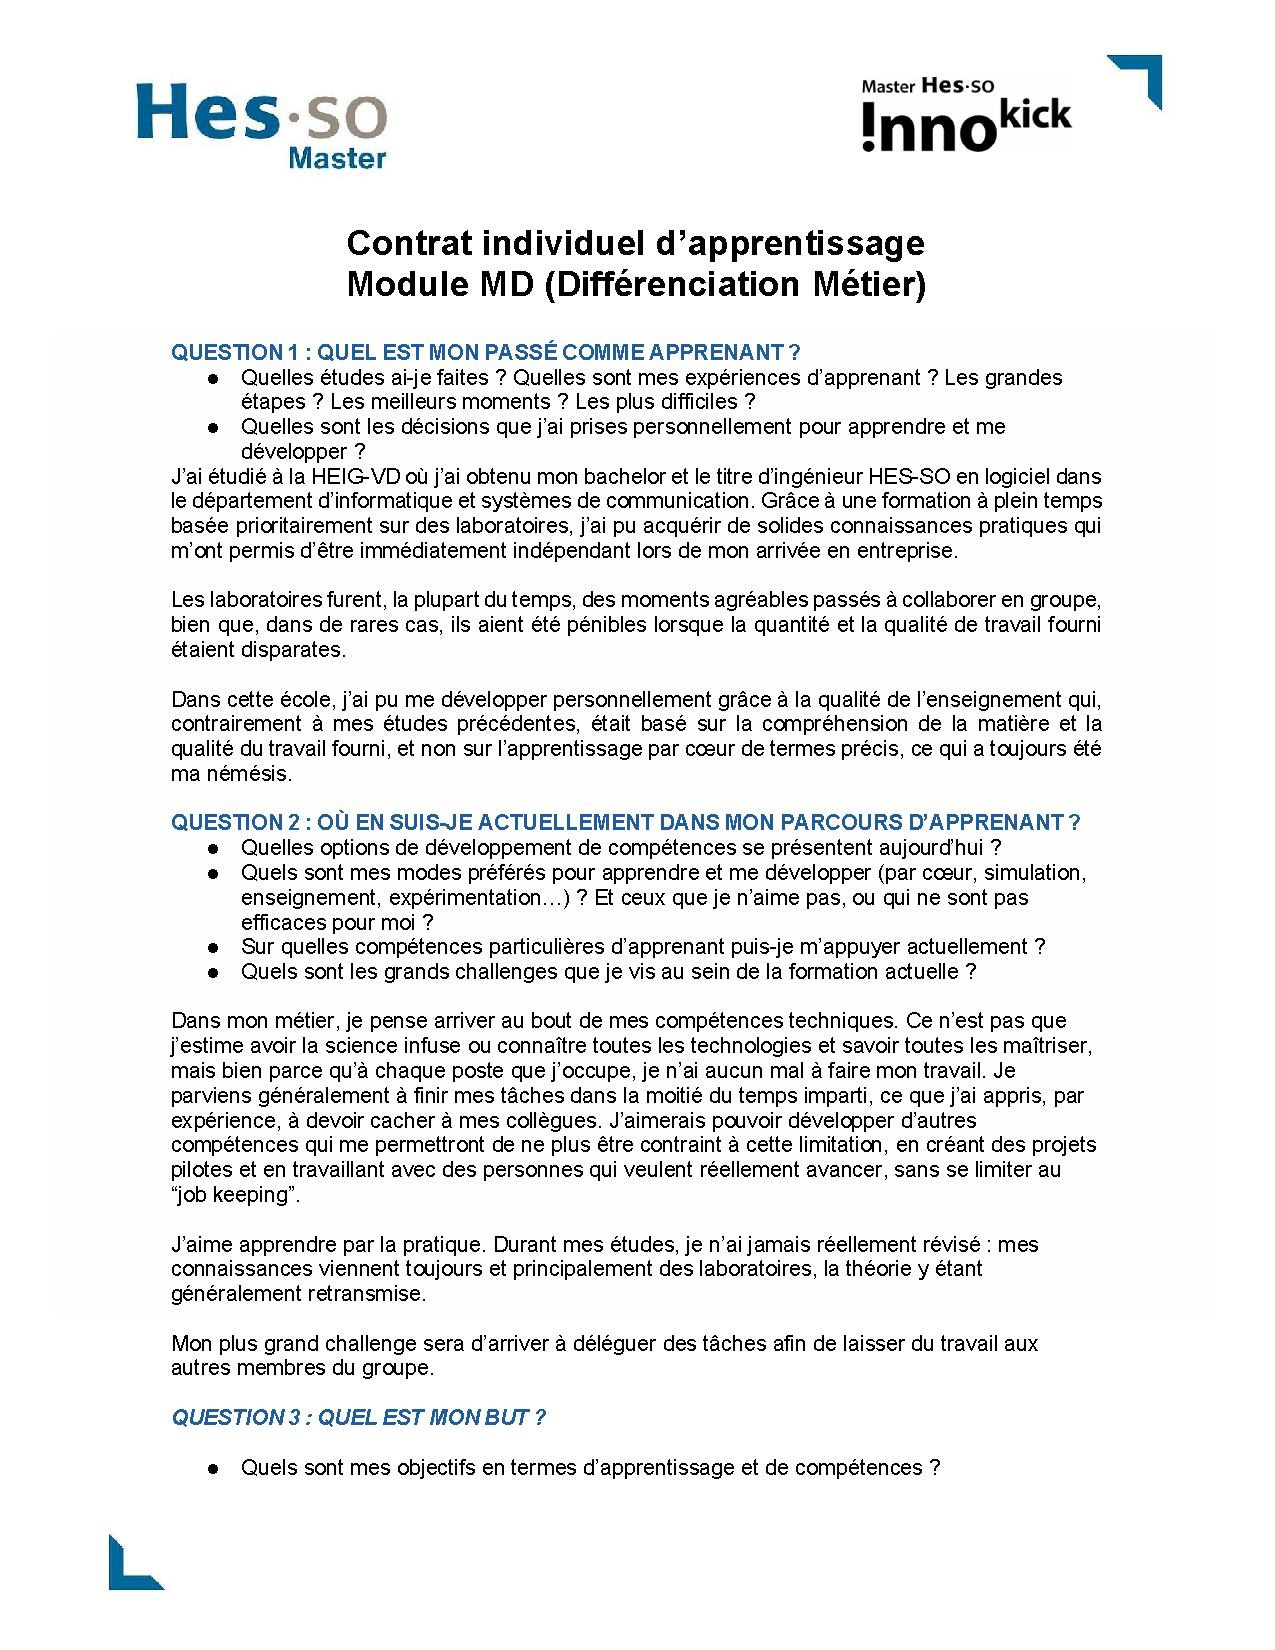
\includepdf[pages=-, pagecommand={\thispagestyle{annexepages}}]{annexes/pdfs/annexe-A-contrat-apprentissage.pdf}

% : Annexe B : Note de décision technique NDT-SW-001 ---
% =============================================================================
% ANNEX B — TECHNICAL DECISION NOTE NDT-SW-001
% =============================================================================

\chapter{Technical Decision Note: NDT-SW-001}
\label{annex:ndt-sw-001}

% --- Note de mise en contexte (portfolio) -------------------------------------
\begin{tcolorbox}[colback=blue!5, colframe=blue!40!black, boxrule=0.5pt, arc=3pt,
  left=8pt, right=8pt, top=6pt, bottom=6pt]
  \small\itshape
  \textbf{Note du portfolio.} Ce document est un artefact professionnel r\'eel,
  produit dans le cadre de la certification IEC~62304 chez TWIICE. Il a \'et\'e
  reformatt\'e en \LaTeX{} afin de pouvoir \^etre int\'egr\'e directement dans
  ce portfolio sous forme de source compilable.

  Conform\'ement aux r\`egles de confidentialit\'e de l'entreprise, les
  informations propres \`a TWIICE (noms des collaborateurs, dates internes,
  signatures) ont \'et\'e \textbf{caviard\'ees} et sont repr\'esent\'ees par
  des barres noires (\caviarder[1.2cm]). Le contenu technique et m\'ethodologique
  du document est, quant \`a lui, int\'egralement reproduit.
\end{tcolorbox}

\bigskip

% --- Document header ----------------------------------------------------------
\begin{tcolorbox}[colback=gray!8, colframe=gray!50, boxrule=0.5pt, arc=3pt,
  left=8pt, right=8pt, top=6pt, bottom=6pt]
  \begin{tabularx}{\linewidth}{@{}p{4.2cm}X@{}}
    \textbf{Reference}          & NDT-SW-001 \\[3pt]
    \textbf{Subject}            & Selection of tooling for SOUP and software artefact traceability \\[3pt]
    \textbf{Applicable standard}& IEC~62304:2006+A1:2015 --- Clause~8 (Software configuration management) \\[3pt]
    \textbf{Author}             & Alexandre Gati --- Software Engineer \\[3pt]
    \textbf{Date}               & \caviarder[2.5cm] \\[3pt]
    \textbf{Status}             & \textbf{Under Review} \\
  \end{tabularx}
\end{tcolorbox}

\bigskip

% ==============================================================================
\section*{1.\quad Context and problem statement}
% ==============================================================================

The TWIICE software team develops the embedded software for a class~IIa medical exoskeleton (MDR Regulation 2017/745). This software incorporates several third-party components (SOUP --- \textit{Software of Unknown Provenance}) whose management is governed by the IEC~62304 standard.

Clause~8 of IEC~62304 mandates a software configuration management system that ensures:

\begin{itemize}
  \item \textbf{Unique identification} of every configuration item (source code, SOUP, build artefacts, documents);
  \item \textbf{Change control} with full traceability;
  \item \textbf{Reproducibility} of any released version of the software;
  \item \textbf{End-to-end traceability}: requirement $\rightarrow$ specification $\rightarrow$ code $\rightarrow$ test $\rightarrow$ release.
\end{itemize}

The team lacked a formalised system meeting these requirements. Several parallel technical debates (processor selection, communication architecture, DevOps tooling) were dispersing collective energy. An Eisenhower matrix prioritisation (cf. Phase~2, Espace modules chapter, in this portfolio) identified SOUP traceability as the \textbf{urgent and important} issue, directly blocking certification.

% ==============================================================================
\section*{2.\quad Options evaluated}
% ==============================================================================

Three options were analysed using a multi-criteria build-vs-buy framework.

\paragraph{Option A --- GitLab (cloud)}
Use of the existing GitLab instance for source code versioning, extended to package registries (GitLab Container Registry, Package Registry) and CI/CD pipelines for automated builds and tests.

\begin{itemize}
  \item \textit{Main advantage}: tool already mastered by the team, marginal cost (included in the existing subscription), immediate deployment.
  \item \textit{Main limitation}: cloud hosting requires a cybersecurity compliance analysis for a medical device.
\end{itemize}

\paragraph{Option B --- Custom solution (in-house development)}
Design and development of a bespoke storage and versioning system, hosted on-premises.

\begin{itemize}
  \item \textit{Main advantage}: full control over format, hosting and security.
  \item \textit{Main limitation}: high development cost (estimate: several person-weeks), ongoing maintenance burden, timeline incompatible with the certification schedule.
\end{itemize}

\paragraph{Option C --- JFrog Artifactory}
Dedicated package manager specialised in binary artefact storage with metadata, checksums and CI/CD integration.

\begin{itemize}
  \item \textit{Main advantage}: native artefact traceability and integrity features.
  \item \textit{Main limitation}: additional licence required, high vendor dependency (proprietary solution).
\end{itemize}

% ==============================================================================
\section*{3.\quad Decision criteria}
% ==============================================================================

The options were assessed against six criteria defined collectively by the software team and the quality team.

\begin{table}[h!]
  \centering\small
  \begin{tabularx}{\textwidth}{|p{3.2cm}|p{2cm}|X|X|X|}
    \hline
    \textbf{Criterion} & \textbf{Weight} & \textbf{GitLab (cloud)} & \textbf{Custom solution} & \textbf{JFrog Artifactory} \\
    \hline
    Integration complexity & High     & \ok{Low}       & \nok{High}          & \warn{Medium} \\
    \hline
    Cost (licence + hours) & High     & \ok{Included}  & \nok{High}          & \warn{Extra licence} \\
    \hline
    IEC~62304 traceability & Critical & \ok{Good}      & \ok{Full}           & \ok{Good} \\
    \hline
    Implementation lead time & High   & \ok{Immediate} & \nok{Weeks/months}  & \ok{A few days} \\
    \hline
    Vendor dependency      & Medium   & \warn{Medium}  & \ok{None}           & \nok{High} \\
    \hline
    Cybersecurity risk     & High     & \warn{Moderate (cloud)} & \ok{Low (on-prem)} & \warn{Moderate (self-hosted possible)} \\
    \hline
  \end{tabularx}
  \caption{Multi-criteria grid --- IEC~62304 configuration management options}
  \label{tab:ndt-criteres}
\end{table}

% ==============================================================================
\section*{4.\quad Analysis and recommendation}
% ==============================================================================

\textbf{Option A (GitLab cloud)} offers the best overall balance:

\begin{itemize}
  \item \textbf{Lead time}: immediate deployment, compatible with the certification schedule.
  \item \textbf{Cost}: zero additional cost (existing subscription).
  \item \textbf{Skills}: tool already mastered by the team, no learning curve.
  \item \textbf{Traceability}: native versioning (tags, releases), package registries, CI/CD pipeline automating tests and builds.
\end{itemize}

Option B (custom) was rejected despite offering full control, due to a timeline and cost incompatible with the resources of a startup in certification phase.

Option C (JFrog) was rejected due to high vendor dependency and additional licence cost, offering marginal functional gain over GitLab in this context.

% ==============================================================================
\section*{5.\quad Selected decision}
% ==============================================================================

\begin{decisionbox}
\textbf{Option A --- GitLab (cloud)}

Use of the existing GitLab instance as the primary software configuration management system, including:

\begin{itemize}
  \item Source code versioning (Git);
  \item Package and build artefact registry (GitLab Package Registry);
  \item CI/CD pipeline for automated unit, integration and artefact generation;
  \item Tags and releases for unique identification of each delivered version.
\end{itemize}
\end{decisionbox}

% ==============================================================================
\section*{6.\quad Residual risks and mitigation measures}
% ==============================================================================

\begin{table}[h!]
  \centering\small
  \begin{tabularx}{\textwidth}{|X|p{2cm}|p{1.8cm}|X|}
    \hline
    \textbf{Risk} & \textbf{Likelihood} & \textbf{Impact} & \textbf{Mitigation} \\
    \hline
    Cloud hosting --- cybersecurity compliance for a medical device
      & Medium & High
      & Vendor compliance analysis (SOC~2, ISO~27001 certifications). Evaluate migration to GitLab self-hosted if required by audit. \\
    \hline
    Vendor dependency --- pricing or terms-of-service change
      & Low & Medium
      & Data exportable (native Git). Migration plan to an alternative (Gitea, GitLab self-hosted) documented. \\
    \hline
    Incomplete traceability --- gap between IEC~62304 requirements and native features
      & Low & High
      & Supplemented by manual documentation (SOUP list, requirements-code-tests traceability matrix). Integrated into the \textit{Definition of Done}. \\
    \hline
    Cloud service availability --- outage impacting development
      & Low & Low
      & Local Git clones on every workstation. Periodic backups of the package registry. \\
    \hline
  \end{tabularx}
  \caption{Residual risks and mitigation measures --- NDT-SW-001}
  \label{tab:ndt-risques}
\end{table}

% ==============================================================================
\section*{8.\quad Approval}
% ==============================================================================

\begin{table}[h!]
  \centering
  \begin{tabular}{|p{4cm}|p{3.5cm}|p{2.5cm}|p{3cm}|}
    \hline
    \textbf{Role} & \textbf{Name} & \textbf{Date} & \textbf{Signature} \\
    \hline
    Author (Software Eng.) & Alexandre Gati     & \caviarder[2cm] & \caviarder[2.5cm] \\[6pt]
    \hline
    Software Architect     & \caviarder[2.5cm]  & \caviarder[2cm] & \caviarder[2.5cm] \\[6pt]
    \hline
    Quality Manager        & \caviarder[2.5cm]  & \caviarder[2cm] & \caviarder[2.5cm] \\[6pt]
    \hline
  \end{tabular}
  \caption{Approval table --- NDT-SW-001}
  \label{tab:ndt-approbation}
\end{table}




% : Annexe C : Extrait du backlog priorisé ---
% =============================================================================
% ANNEX C — PRIORITISED BACKLOG EXTRACT
% =============================================================================

\chapter{Prioritised Backlog Extract}
\label{annex:backlog}

% --- Note de mise en contexte (portfolio) -------------------------------------
\begin{tcolorbox}[colback=blue!5, colframe=blue!40!black, boxrule=0.5pt, arc=3pt,
  left=8pt, right=8pt, top=6pt, bottom=6pt]
  \small\itshape
  \textbf{Note du portfolio.} Ce document est un extrait du backlog de
  l'\'equipe logicielle TWIICE, export\'e depuis le board GitLab du projet.
  Il illustre la hi\'erarchisation des t\^aches apr\`es application de la
  matrice d'Eisenhower (cf. Phase~2, Espace modules du pr\'esent portfolio).

  Conform\'ement aux r\`egles de confidentialit\'e de l'entreprise, les
  informations sensibles (num\'eros d'issues, noms des collaborateurs, dates,
  jalons internes) ont \'et\'e \textbf{caviard\'ees} et sont repr\'esent\'ees
  par des barres noires (\caviarder[1.2cm]). Les intitul\'es des t\^aches et
  leur description technique sont, quant \`a eux, int\'egralement reproduits.
\end{tcolorbox}

\bigskip

% --- Sprint / Project header --------------------------------------------------
\begin{tcolorbox}[colback=gray!8, colframe=gray!50, boxrule=0.5pt, arc=3pt,
  left=8pt, right=8pt, top=6pt, bottom=6pt]
  \begin{tabularx}{\linewidth}{@{}p{4cm}X@{}}
    \textbf{Project}   & TWIICE Exoskeleton --- Software \\[3pt]
    \textbf{Milestone} & \caviarder[3cm] \\[3pt]
    \textbf{Sprint}    & \caviarder[2cm]\quad
                         (\caviarder[2cm]\;--\;\caviarder[2cm]) \\[3pt]
    \textbf{Board}     & \caviarder[5cm] \\[3pt]
    \textbf{Exported by} & Alexandre Gati \\[3pt]
    \textbf{Export date} & \caviarder[2.5cm] \\
  \end{tabularx}
\end{tcolorbox}

\bigskip

% ==============================================================================
\section*{Context}
% ==============================================================================

The following extract lists the software issues identified and re-prioritised
following an Eisenhower matrix exercise conducted with the team (see Annex~B,
\S1). Issues are grouped by priority level --- \highprio, \mediumprio,
\lowprio{} --- and ordered within each group by creation date. Redacted fields
(\caviarder[0.9cm]) contain information covered by the company's
confidentiality policy.

\bigskip

% ==============================================================================
% BACKLOG TABLE
% ==============================================================================

\begingroup
\setlength{\tabcolsep}{3pt}
\begin{table}[h!]
  \centering\footnotesize
  \begin{tabularx}{\textwidth}{|p{1.4cm}|p{1.1cm}|X|p{2.0cm}|p{1.4cm}|p{1.7cm}|}
    \hline
    \rowcolor{gray!15}
    \textbf{Priority} & \textbf{Issue\,\#} & \textbf{Title \& description} &
    \textbf{Assignee} & \textbf{Due} & \textbf{Status} \\
    \hline

    % ------------------------------------------------------------------
    % HIGH PRIORITY
    % ------------------------------------------------------------------

    \highprio
      & \caviarder[0.8cm]
      & \textbf{Set up SOUP traceability --- GitLab Package Registry}
        \newline{\footnotesize
          Register all third-party libraries (SOUP list) in the GitLab Package
          Registry. Ensure each entry includes version, licence, source URL and
          checksum, per IEC~62304 \S8.1.2.
          \newline\textit{Labels:} \texttt{iec-62304}, \texttt{certification},
          \texttt{sprint-\caviarder[0.4cm]}}
      & \caviarder[2.2cm]
      & \caviarder[1.5cm]
      & \sinprogress \\
    \hline

    \highprio
      & \caviarder[0.8cm]
      & \textbf{Document all third-party components (IEC~62304 \S8)}
        \newline{\footnotesize
          Produce the SOUP list artefact required by IEC~62304 clause~8:
          component name, version, publisher, risk classification.
          Cross-reference with the software requirements specification.
          \newline\textit{Labels:} \texttt{iec-62304}, \texttt{documentation},
          \texttt{sprint-\caviarder[0.4cm]}}
      & \caviarder[2.2cm]
      & \caviarder[1.5cm]
      & \sinprogress \\
    \hline

    \highprio
      & \caviarder[0.8cm]
      & \textbf{Define CI/CD pipeline --- automated build \& test artefacts}
        \newline{\footnotesize
          Configure the GitLab CI pipeline to produce reproducible build
          artefacts (binary, SBOM, test report) and publish them to the
          Package Registry with immutable versioning tags.
          \newline\textit{Labels:} \texttt{ci-cd}, \texttt{iec-62304},
          \texttt{sprint-\caviarder[0.4cm]}}
      & \caviarder[2.2cm]
      & \caviarder[1.5cm]
      & \stodo \\
    \hline

    % ------------------------------------------------------------------
    % MEDIUM PRIORITY
    % ------------------------------------------------------------------

    \mediumprio
      & \caviarder[0.8cm]
      & \textbf{Standardise documentation templates (IEC~62304)}
        \newline{\footnotesize
          Create shared GitLab Wiki templates for: SOUP list, change request,
          software release note, design review record. Reduces manual overhead
          and ensures consistent artefact format across sprints.
          \newline\textit{Labels:} \texttt{documentation},
          \texttt{sprint-\caviarder[0.4cm]}}
      & \caviarder[2.2cm]
      & \caviarder[1.5cm]
      & \stodo \\
    \hline

    \mediumprio
      & \caviarder[0.8cm]
      & \textbf{Update SOUP risk assessment --- IEC~62304 \S7.2}
        \newline{\footnotesize
          Review existing risk assessments for embedded SOUP (FreeRTOS,
          libmodbus, \caviarder[1.5cm]). Align severity classifications with
          the updated device risk file (MDR class~IIa context).
          \newline\textit{Labels:} \texttt{risk}, \texttt{iec-62304}}
      & \caviarder[2.2cm]
      & \caviarder[1.5cm]
      & \sbacklog \\
    \hline

    % ------------------------------------------------------------------
    % LOW PRIORITY
    % ------------------------------------------------------------------

    \lowprio
      & \caviarder[0.8cm]
      & \textbf{Evaluate MCU vs Jetson for user interface module}
        \newline{\footnotesize
          Comparative benchmark: processing power, energy budget, SDK
          maturity, lead time. Decision deferred --- not blocking
          certification. To be scheduled post-milestone
          \caviarder[1.2cm].
          \newline\textit{Labels:} \texttt{hardware}, \texttt{research}}
      & \caviarder[2.2cm]
      & \caviarder[1.5cm]
      & \sbacklog \\
    \hline

    \lowprio
      & \caviarder[0.8cm]
      & \textbf{Benchmark supplementary DevOps tools}
        \newline{\footnotesize
          Evaluate JFrog Artifactory, Nexus Repository and Harbor as
          potential complements to the GitLab Package Registry. No
          blocker identified --- team comfort improvement only.
          \newline\textit{Labels:} \texttt{devops}, \texttt{tooling}}
      & \caviarder[2.2cm]
      & \caviarder[1.5cm]
      & \sbacklog \\
    \hline

  \end{tabularx}
  \caption{Prioritised backlog extract --- TWIICE Software, post-Eisenhower
    matrix triage}
  \label{tab:backlog}
\end{table}
\endgroup

% ==============================================================================
\section*{Traceability to the Eisenhower matrix}
% ==============================================================================

The table below maps each priority group to the corresponding quadrant of the
Eisenhower matrix applied during the Phase~2 (Definition) workshop.

\begin{table}[h!]
  \centering\small
  \begin{tabularx}{\textwidth}{|p{1.6cm}|p{3.5cm}|X|}
    \hline
    \textbf{Priority} & \textbf{Eisenhower quadrant} & \textbf{Rationale} \\
    \hline
    \highprio
      & Urgent \& Important
      & Directly blocks the IEC~62304 certification audit. Must be resolved
        within the current or immediately following sprint. \\
    \hline
    \mediumprio
      & Important, not urgent
      & Required for long-term compliance and team efficiency, but does not
        block the next certification milestone. Scheduled in upcoming sprints. \\
    \hline
    \lowprio
      & Not important (current context)
      & Debated actively during the workshop but identified as non-blocking.
        Deferred to the post-certification backlog. \\
    \hline
  \end{tabularx}
  \caption{Mapping between backlog priority levels and Eisenhower quadrants}
  \label{tab:backlog-eisenhower}
\end{table}







% : Annexe D : Software Development Plan (reproduction markdown caviardee) ---
% =============================================================================
% ANNEX D : SOFTWARE DEVELOPMENT PLAN (FORMALIZED AND REDACTED VERSION)
% =============================================================================

\chapter{Software Development Plan (formalized and redacted version)}
\label{annex:sdp-markdown}

\begin{tcolorbox}[colback=blue!5, colframe=blue!40!black, boxrule=0.5pt, arc=3pt,
  left=8pt, right=8pt, top=6pt, bottom=6pt]
  \small\itshape
  \textbf{Avertissement.} Le contenu ci-dessous est une reproduction formalisee en \LaTeX{} du Software Development Plan original. Cette version a ete volontairement \textbf{tronquee} et caviardee afin de proteger les informations sensibles (identites, identifiants documentaires internes, liens, details d'infrastructure et metadonnees de pilotage). Des notes de bas de page explicatives ont egalement ete ajoutees pour en faciliter la lecture par un public \textbf{novice}.
\end{tcolorbox}

\section*{1. Document control}

\subsection*{1.1 Roles}
\begin{tabularx}{\textwidth}{|p{3.3cm}|p{2.5cm}|X|p{3cm}|}
\hline
\textbf{Role} & \textbf{Name} & \textbf{Reason for signature} & \textbf{Signature \& date} \\
\hline
System Quality Manager & \caviarder[2.8cm] & Document Owner, Author & \caviarder[2.8cm] \\
\hline
Software Engineer & \caviarder[2.8cm] & Reviewer & \caviarder[2.8cm] \\
\hline
Software Manager & \caviarder[2.8cm] & Approver & \caviarder[2.8cm] \\
\hline
\end{tabularx}

\subsection*{1.2 Version history}
\begin{tabularx}{\textwidth}{|p{2.5cm}|X|}
\hline
\textbf{Version} & \textbf{Description} \\
\hline
1 & Initial version \\
\hline
\end{tabularx}

\subsection*{1.3 References (redacted)}
\begin{longtable}{|p{1.4cm}|p{12cm}|}
\hline
\textbf{Ref.} & \textbf{Document} \\
\hline
R1 & Internal controlled procedure (\caviarder[5.2cm]) \\
\hline
R2 & Internal controlled procedure (\caviarder[5.2cm]) \\
\hline
R3 & Internal controlled procedure (\caviarder[5.2cm]) \\
\hline
R4 & Internal controlled procedure (\caviarder[5.2cm]) \\
\hline
R5 & IEC~62304:2006+AMD1:2015, Medical device software life cycle processes \\
\hline
R6 & Internal controlled procedure (\caviarder[5.2cm]) \\
\hline
R7 & Internal controlled procedure (\caviarder[5.2cm]) \\
\hline
R8 & Internal controlled procedure (\caviarder[5.2cm]) \\
\hline
R9 & Internal controlled procedure (\caviarder[5.2cm]) \\
\hline
R10 & Internal controlled procedure (\caviarder[5.2cm]) \\
\hline
R11 & FDA: Content of Premarket Submissions for Device Software Functions \\
\hline
R12-R19 & Internal project documents (plans, architecture, risk records, detailed design): \caviarder[3.4cm] \\
\hline
\end{longtable}

\subsection*{1.4 Definitions (extract)}
\begin{longtable}{|p{3cm}|p{10.4cm}|}
\hline
\textbf{Term} & \textbf{Definition} \\
\hline
Software System & Integrated collection of Software Items organized to accomplish a function set (IEC~62304 3.28). \\
\hline
Software Item & Any identifiable part of a computer program (IEC~62304 3.25). \\
\hline
Software Unit & Software Item not subdivided into other items (IEC~62304 3.29). \\
\hline
SOUP / OTS & Third-party software not fully controlled through manufacturer life cycle. \\
\hline
SDP & Software Development Plan. \\
\hline
SRS & Software Requirements Specification: defines what software shall do. \\
\hline
SDDD & Software Detailed Design Document: internal design of software items/units. \\
\hline
Software Anomaly & Condition deviating from expected behavior. \\
\hline
\end{longtable}

\section*{2. Purpose and scope}

The SDP defines software development processes for the medical device in compliance with IEC~62304 and internal controlled procedures (\caviarder[2.8cm]).

\subsection*{2.1 Scope}
The plan covers software components in scope: \caviarder[5.5cm].

The document is reviewed at each Gate Review (G1 to G4) and updated under formal change control.

\section*{3. Software safety classification}

\textbf{Preliminary classification:} \caviarder[2.2cm] (conservative assumption for an active medical device).

\textbf{Segregation strategy:}
\begin{itemize}
  \item Critical control loops handled as \caviarder[1.8cm].
  \item Auxiliary applications potentially classified as \caviarder[2.4cm] if architectural segregation is demonstrated.
\end{itemize}

\section*{4. Roles and responsibilities (extrait)}

\begin{tabularx}{\textwidth}{|p{3cm}|X|p{3cm}|}
\hline
\textbf{Role} & \textbf{Responsibilities} & \textbf{Assigned to} \\
\hline
Software Lead & Executes the SDP, arbitrates architecture, and coordinates verification and change impacts. & \caviarder[2.8cm] \\
\hline
Software Developer & Development, unit testing, static analysis, and merge requests. & \caviarder[2.8cm] \\
\hline
Configuration Manager & SCM, CI/CD pipelines, SOUP management, and release baselines. & \caviarder[2.8cm] \\
\hline
Quality Manager & Traceability review, gate validation, and SOP compliance. & \caviarder[2.8cm] \\
\hline
Risk Manager & RMF follow-up\footnote{\textbf{RMF} stands for \textit{Risk Management File}. It contains the records documenting risk analysis, risk control measures, and their verification evidence.}, and safety-impact review of anomalies and changes. & \caviarder[2.8cm] \\
\hline
\end{tabularx}

\section*{5. Development life cycle model}

The project follows a V-Model integrated into the Stage-Gate process.

\begin{tabularx}{\textwidth}{|p{1.2cm}|p{2.2cm}|p{2.5cm}|X|}
\hline
\textbf{Gate} & \textbf{Phase} & \textbf{IEC~62304} & \textbf{Key software activities} \\
\hline
G0 & Planning & 5.1 & User need definition (\caviarder[2.8cm]) \\
\hline
G1 & Input \& Arch. & 5.1, 5.2, 5.3 & SDP, SRS\footnote{\textbf{SRS} stands for \textit{Software Requirements Specification}. This document formalizes verifiable software requirements.}, \caviarder[3.8cm] \\
\hline
G2 & Detailed design & 5.4, 5.5 & SDDD\footnote{\textbf{SDDD} stands for \textit{Software Detailed Design Document}. It decomposes architecture into implementable and testable components/units.}, \caviarder[4.6cm] \\
\hline
G3 & Verification & 5.6, 5.7 & Integration, system testing, \caviarder[2.8cm] \\
\hline
G4 & Validation & 5.8 & Software release and \caviarder[2.4cm] \\
\hline
\end{tabularx}

\medskip
\textbf{Planned deviation:} SDP produced at G1 (instead of G0), since \caviarder[5.8cm].

\section*{6. Traceability and verification framework}

\textbf{Traceability rules:}
\begin{itemize}
  \item Each software requirement has an upstream link to a system requirement and/or risk control measure.
  \item Each software requirement has downstream links to design, code, and verification activity.
  \item Completeness review is performed before each gate.
\end{itemize}

\textbf{Verification strategy (summary):}
\begin{tabularx}{\textwidth}{|p{1.2cm}|p{3.1cm}|X|}
\hline
\textbf{Gate} & \textbf{Verification activity} & \textbf{Acceptance criteria} \\
\hline
G1 & Design review & Requirements and architecture are baselined; \caviarder[3.6cm] \\
\hline
G2 & Unit verification & Static analysis compliant, \caviarder[3.8cm] \\
\hline
G3 & Integration \& system verification & Requirement coverage and integration/system tests validated, \caviarder[2.8cm] \\
\hline
G4 & Release verification & Release package complete; \caviarder[3.4cm] \\
\hline
\end{tabularx}

\section*{7. Software configuration management (SCM)}

SCM is aligned with internal controlled procedures (\caviarder[2.2cm]) using a controlled branching strategy.

\begin{itemize}
  \item \caviarder[2.6cm]: release baseline, direct commits prohibited.
  \item \caviarder[2.6cm]: continuous integration of evolutions.
  \item \caviarder[2.6cm]: preparation of official versions.
  \item \caviarder[2.6cm]: post-release correction with impact analysis.
  \item \caviarder[3.8cm]: development branches.
\end{itemize}

\section*{8. SOUP, cybersecurity, release and maintenance}

\textbf{SOUP management:}
\begin{itemize}
  \item SOUP inventory maintained and periodically reviewed.
  \item SOUP components verified through test plans.
  \item Vulnerability and end-of-life monitoring performed continuously.
\end{itemize}

\textbf{Release:}
release includes version, hash, residual anomalies, SOUP components, and \caviarder[3.8cm], followed by controlled archiving.

\textbf{Problem resolution and maintenance:}
each anomaly follows a documented cycle: logging, triage, investigation, resolution, regression check, then traceability to \caviarder[3.2cm].

\section*{9. Deliverables matrix (redacted summary)}

\begin{tabularx}{\textwidth}{|X|p{2.4cm}|p{1.5cm}|p{2.1cm}|}
\hline
\textbf{Deliverable} & \textbf{Format} & \textbf{Gate} & \textbf{IEC~62304} \\
\hline
SDP & \caviarder[2.2cm] signed & G1 & 5.1 \\
\hline
SRS / Architecture & \caviarder[2.2cm] signed & G1 & 5.2 / 5.3 \\
\hline
SDDD + unit evidence & \caviarder[3.2cm] + PDF signed & G2 & 5.4 / 5.5 \\
\hline
Integration/System tests + traceability matrix & \caviarder[2.6cm] & G3 & 5.6 / 5.7 \\
\hline
Release notes + final SOUP list + software RMF section & \caviarder[2.6cm] & G4 & 5.8 / clause 7 \\
\hline
\end{tabularx}

\medskip
\noindent\textit{Note: detailed document identifiers, storage links, internal audit trails, and operational references are redacted in this portfolio version.}





% : Annexe E : Journal réflexif ---
\chapter{Journal réflexif : Master Innokick}
\label{annex:journal-reflexif}
\annexefiche
  {Entrées produites au fil de l'année académique 2025--2026}
  {Journal personnel de suivi des apprentissages (cours, situations, prises de recul)}
  {Fond réflexif transversal mobilisé dans les analyses A2/B4/C2 et dans le chapitre \textit{Perspectives}}
  {Caviardage léger : éventuelles données sensibles personnelles ou tierces}
\includepdf[pages=-, pagecommand={\thispagestyle{annexepages}}]{annexes/pdfs/annexe-E-journal-reflexif.pdf}

% : Annexe F : Compte-rendu de la première rétrospective (B4) ---
% =============================================================================
% ANNEX F : TEAM RETROSPECTIVE REPORT (B4), REDACTED
% =============================================================================

\chapter{First team retrospective report (B4)}
\label{annex:retro-b4}

\begin{tcolorbox}[colback=blue!5, colframe=blue!40!black, boxrule=0.5pt, arc=3pt,
  left=8pt, right=8pt, top=6pt, bottom=6pt]
  \small\itshape
  \textbf{Avertissement.} Cette annexe est une reproduction \textbf{non fidele} d'un compte-rendu de retrospective utilise en contexte professionnel. Elle est volontairement adaptee, tronquee et caviardee a des fins de \textbf{demonstration} et de \textbf{preuve} dans le portfolio. Les informations sensibles (identites, dates exactes, identifiants, references internes et metadonnees d'outillage) ont ete masquees.
\end{tcolorbox}

\bigskip

\begin{tcolorbox}[colback=gray!8, colframe=gray!50, boxrule=0.5pt, arc=3pt,
  left=8pt, right=8pt, top=6pt, bottom=6pt]
\begin{tabularx}{\linewidth}{@{}p{4.3cm}X@{}}
\textbf{Team} & TWIICE software team \\
\textbf{Related sprint} & Sprint \caviarder[1.8cm] (2 weeks) \\
\textbf{Retrospective date} & \caviarder[2.2cm] \\
\textbf{Facilitator} & \caviarder[2.6cm] \\
\textbf{Participants} & \caviarder[6cm] \\
\textbf{Context} & First complete retrospective after deployment of an IEC~62304-adapted agile framework \\
\end{tabularx}
\end{tcolorbox}

\section*{1. Retrospective objective}

Evaluate the sprint across three axes: what should continue, what should stop, and what should start in the next sprint. The operational goal is to improve agile delivery pace while strengthening certification-grade documentation quality.

\section*{2. Method applied}

The session follows a Start/Stop/Continue format, with timeboxing, collective priority voting, and final action validation. Each retained action is assigned an owner, a deadline, and a verification criterion.

\section*{3. Start / Stop / Continue results}

\begin{tabularx}{\textwidth}{|p{2.2cm}|X|}
\hline
\textbf{Continue} &
\begin{itemize}
  \item Maintain the 15-minute daily ritual focused on technical blockers and compliance risks.
  \item Keep the value $\times$ certification-risk prioritization model in the backlog.
  \item Continue cross-review between development and quality before sprint closure.
\end{itemize} \\
\hline
\textbf{Stop} &
\begin{itemize}
  \item Stop late end-of-sprint merges without complete documentation checks.
  \item Stop ambiguous tickets without explicit acceptance criteria.
  \item Stop ad hoc anomaly handling outside the prioritized queue.
\end{itemize} \\
\hline
\textbf{Start} &
\begin{itemize}
  \item Start a single DoD checklist (code, tests, IEC~62304 docs, quality review).
  \item Start a standardized "residual risks" section in each decision note.
  \item Start weekly monitoring of traceability gaps (requirements $\rightarrow$ tests $\rightarrow$ evidence).
\end{itemize} \\
\hline
\end{tabularx}

\section*{4. Retained actions and execution evidence}

\begin{tabularx}{\textwidth}{|p{4.6cm}|p{2.7cm}|p{2.4cm}|X|}
\hline
\textbf{Action} & \textbf{Owner} & \textbf{Deadline} & \textbf{Verification criterion} \\
\hline
Common DoD checklist activated on all tickets in the next sprint & \caviarder[2.1cm] & \caviarder[1.8cm] & 100\% of "Done" tickets include code + tests + documented traceability \\
\hline
"Residual risks" template added to decision notes & \caviarder[2.1cm] & \caviarder[1.8cm] & Each new decision note includes risks + mitigation section \\
\hline
Weekly traceability review institutionalized & \caviarder[2.1cm] & \caviarder[1.8cm] & Gap dashboard maintained; critical gaps closed before gate review \\
\hline
\end{tabularx}

\section*{5. How this evidence demonstrates training impact}

This retrospective evidences a change in maturity level.

\begin{itemize}
  \item \textbf{Before training}: verbal feedback loops, weak traceability, and limited action follow-through.
  \item \textbf{After training}: explicit improvement loop (observation $\rightarrow$ action $\rightarrow$ verification) with auditable artifacts.
\end{itemize}

The observable benefit is twofold: team dynamics become more stable (fewer repeated debates), and compliance becomes integrated into daily steering rather than appended at end of cycle.

\section*{6. Closure status}

\begin{tabularx}{\textwidth}{|p{4.2cm}|X|}
\hline
\textbf{Team validation} & Retrospective approved by the project team (redacted trace) \\
\hline
\textbf{Documentation trace} & Record linked to sprint artifacts \caviarder[2.0cm] and to gate preparation \caviarder[1.6cm] \\
\hline
\textbf{Link to B4 competency} & Evidence of genuine iterative adaptation in a regulated environment \\
\hline
\end{tabularx}




% : Annexe G : Package de priorisation C2 ---
% =============================================================================
% ANNEX G : C2 PRIORITIZATION PACKAGE (MATRIX + WORKSHOP + ROADMAP)
% =============================================================================

\chapter{C2 package: prioritization, workshop, and roadmap}
\label{annex:c2-priorisation}

\begin{tcolorbox}[colback=blue!5, colframe=blue!40!black, boxrule=0.5pt, arc=3pt,
  left=8pt, right=8pt, top=6pt, bottom=6pt]
  \small\itshape
  \textbf{Avertissement.} Cette annexe est une reproduction \textbf{non fidele} d'artefacts de synthese mobilises pour la competence C2. Elle est volontairement adaptee, tronquee et caviardee a des fins de \textbf{demonstration} et de \textbf{preuve} dans le portfolio. Les informations sensibles (identites, identifiants internes, references d'outillage et metadonnees projet) ont ete masquees.
\end{tcolorbox}

\section*{1. Prioritization matrix for evolutions}

\begin{tabularx}{\textwidth}{|p{3.1cm}|X|X|}
\hline
 & \textbf{High feasibility} & \textbf{Low/medium feasibility} \\
\hline
\textbf{High user impact}
&
\begin{itemize}
  \item Assisted-walking mode stability (Must)
  \item Sensor calibration reliability (Must)
\end{itemize}
&
\begin{itemize}
  \item Telemetry pipeline redesign \caviarder[1.8cm] (Should)
\end{itemize} \\
\hline
\textbf{Medium user impact}
&
\begin{itemize}
  \item Coach screen UX optimization (Should)
\end{itemize}
&
\begin{itemize}
  \item Architecture evolution \caviarder[1.8cm] (Could)
\end{itemize} \\
\hline
\textbf{Low user impact}
&
\begin{itemize}
  \item Cosmetic interface adjustments (Could)
\end{itemize}
&
\begin{itemize}
  \item Exploratory work outside sprint scope (Won't now)
\end{itemize} \\
\hline
\end{tabularx}

\medskip
\noindent\textbf{Result.} The matrix reduced a portfolio of approximately 150 requests to a prioritized core of \caviarder[1.1cm] action streams validated in workshop.

\section*{2. Workshop report: problem-definition convergence}

\begin{tcolorbox}[colback=gray!8, colframe=gray!50, boxrule=0.5pt, arc=3pt,
  left=8pt, right=8pt, top=6pt, bottom=6pt]
\begin{tabularx}{\linewidth}{@{}p{4.3cm}X@{}}
\textbf{Date} & \caviarder[2.3cm] \\
\textbf{Participants} & Software team, quality team, usage representatives \caviarder[2.2cm] \\
\textbf{Facilitator} & \caviarder[2.6cm] \\
\textbf{Objective} & Move from raw requests to 3--5 prioritized and actionable problem statements \\
\end{tabularx}
\end{tcolorbox}

\textbf{Problem statement 1 (high priority).}
Secure reliability of critical functions before extending secondary features.

\textbf{Problem statement 2 (high priority).}
Reduce lead time for blocking-anomaly handling by clarifying ownership and prioritization criteria.

\textbf{Problem statement 3 (medium priority).}
Improve readability of technical decisions to reduce cross-team debate reopenings.

\medskip
\noindent\textbf{Convergence mechanism.} Each retained problem statement is selected through structured voting, then reformulated into a shared problem sentence validated by all attending stakeholders.

\section*{3. Roadmap derived from prioritization}

\begin{tabularx}{\textwidth}{|p{3.7cm}|p{2.3cm}|X|p{2.1cm}|}
\hline
\textbf{Axis} & \textbf{Horizon} & \textbf{Operational objective} & \textbf{Indicator} \\
\hline
Critical-function reliability & Sprint S+1 to S+2 & Close critical tickets linked to assisted-walking stability & Closure rate >= \caviarder[1.1cm] \\
\hline
Anomaly flow and prioritization & Sprint S+1 & Implement weekly triage ritual + MoSCoW ranking rule & Average triage delay <= \caviarder[1.4cm] \\
\hline
Decision traceability & Sprint S+1 to S+3 & Standardize decision note + backlog linkage + verification evidence & 100\% of major decisions traceable \\
\hline
\end{tabularx}

\section*{4. Why this annex evidences competency C2}

This annex shows a complete chain:
\begin{enumerate}
  \item raw-request collection,
  \item matrix-based synthesis,
  \item workshop convergence,
  \item translation into a measurable roadmap.
\end{enumerate}

The decisive C2 evidence is the transformation of a heterogeneous request volume into prioritized, shared, and time-steerable problem statements.




% : Annexe H : Descriptif de module Différenciation métier ---
\chapter{Descriptif de module : Différenciation métier (MDM)}
\label{annex:descriptif-mdm}
\annexefiche
  {Version institutionnelle en vigueur pendant l'année 2025--2026}
  {Document officiel HES-SO Innokick -- cadre pédagogique du module MDM}
  {Justification du périmètre d'évaluation, articulation des attendus et positionnement des preuves du portfolio}
  {Aucun caviardage (document institutionnel public)}
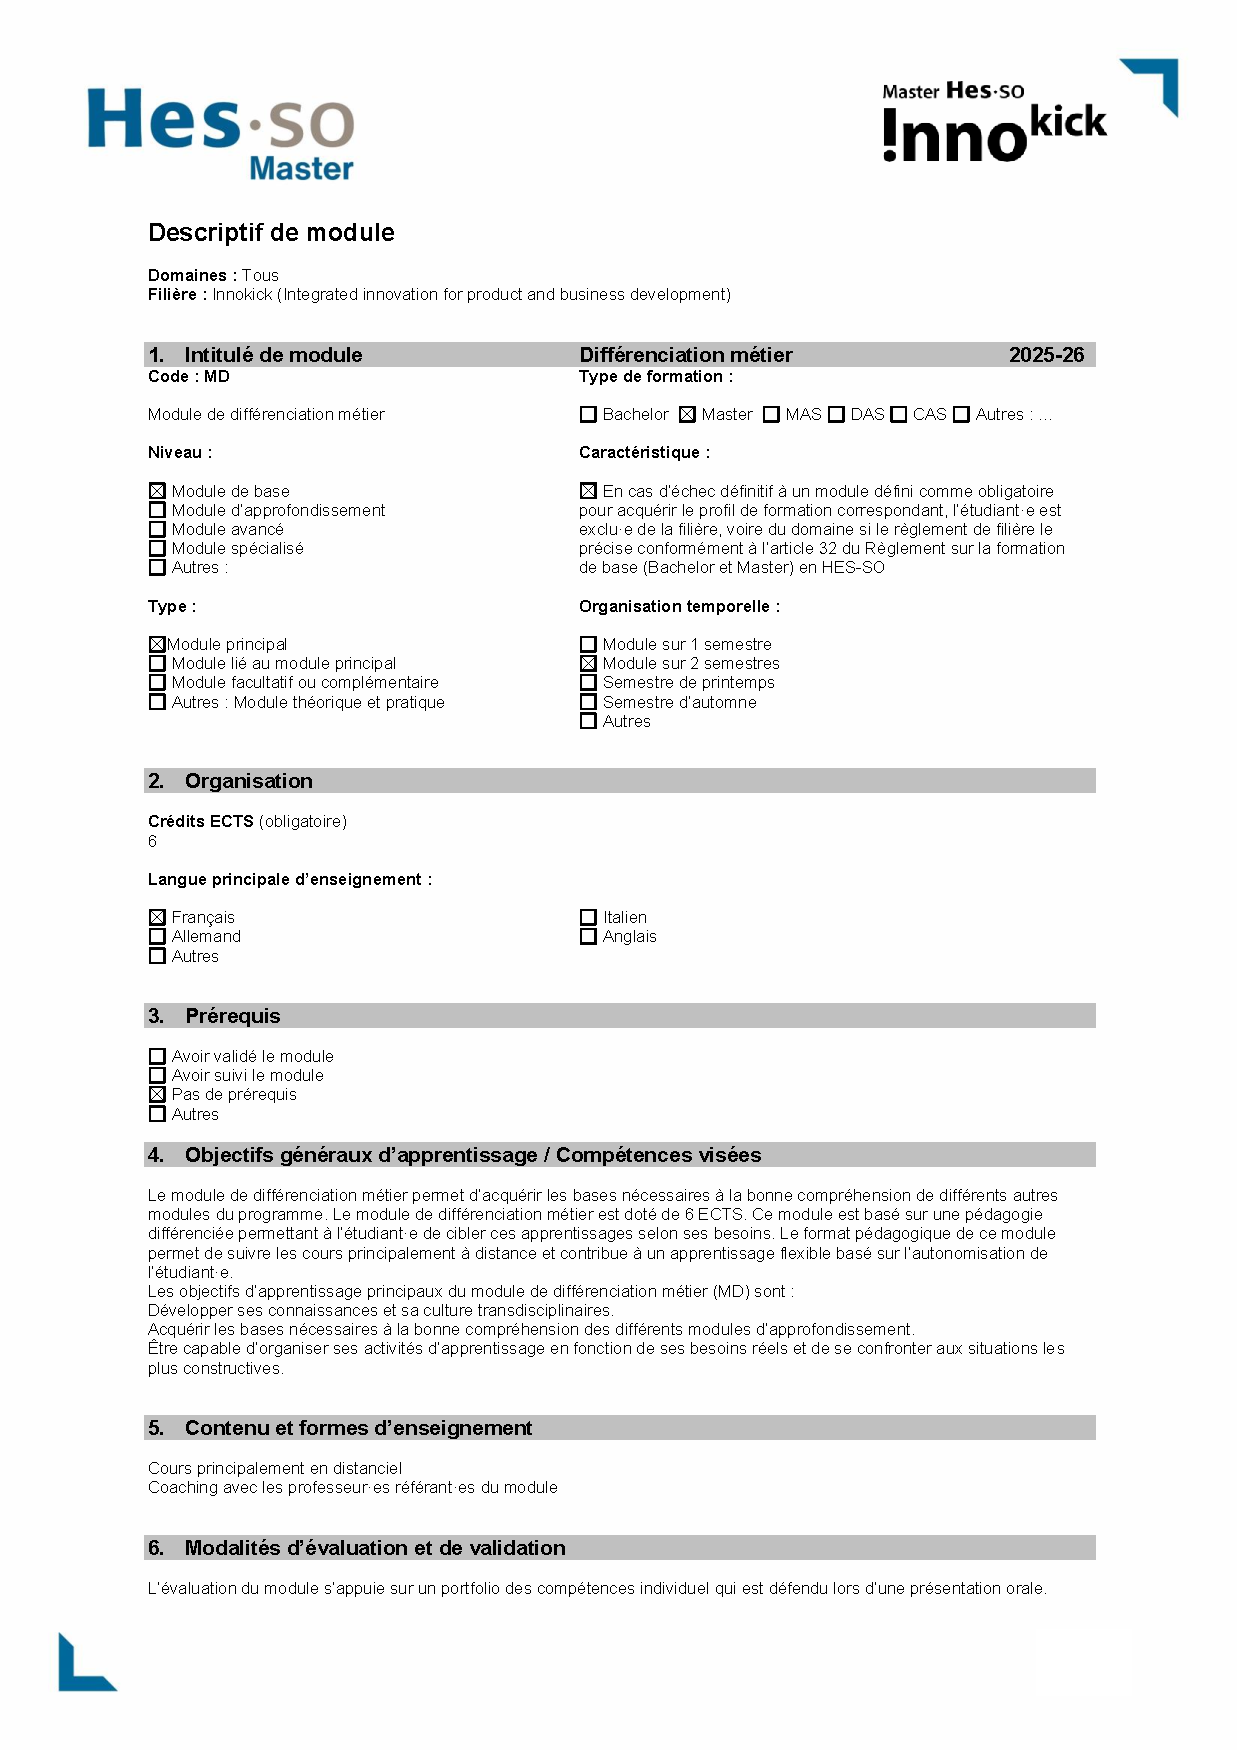
\includepdf[pages=-, pagecommand={\thispagestyle{annexepages}}]{annexes/pdfs/annexe-H-descriptif-mdm.pdf}

% : Annexe I : Plan d'Études Cadre (PEC) Master HES-SO Innokick ---
\chapter{Plan d'Études Cadre (PEC) : Master HES-SO Innokick (07.2024)}
\label{annex:pec-innokick}
\annexefiche
  {Version officielle juillet 2024 (document de référence programme)}
  {Cadre institutionnel global du Master HES-SO Innokick}
  {Fondement normatif des compétences, des phases Design Thinking et de la justification de périmètre (phase 6)}
  {Aucun caviardage (document institutionnel public)}

\includepdf[pages=-, pagecommand={\thispagestyle{annexepages}}]{annexes/pdfs/annexe-I-pec-innokick.pdf}

% : Annexe J : Glossaire technique ---
% =============================================================================
% ANNEXE J : Glossaire technique
% =============================================================================
% Consolide les définitions des termes techniques répétés dans le corps du
% portfolio (footnotes) afin d'alléger la lecture et de fournir une référence
% unique consultable de manière transversale.
% =============================================================================

\chapter{Glossaire technique}
\label{annex:glossaire}

\annexefiche
  {Consolidation produite en 2026 à partir des notes de bas de page du portfolio}
  {Référentiel transversal de vocabulaire technique utilisé dans les chapitres analytiques}
  {Lisibilité et précision terminologique (soutien transversal A2/B4/C2)}
  {Aucun caviardage (document pédagogique consolidé)}

Ce glossaire regroupe les définitions des termes techniques mobilisés dans le portfolio. Il vise à offrir une référence unique consultable de manière transversale, sans nécessiter le retour à chaque note de bas de page. Les termes sont classés par ordre alphabétique.

\bigskip

\begin{description}
  \item[\textbf{Agile (méthodes)}] Approches de gestion de projet fondées sur des cycles courts, la collaboration et l'adaptation continue. Elles privilégient des livraisons incrémentales plutôt qu'une planification figée.

  \item[\textbf{Architecture (logicielle)}] Organisation structurelle d'un système logiciel : découpage des composants, agencement, mise en relation, décisions techniques régissant leurs interactions (protocoles, interfaces, gestion des états).

  \item[\textbf{Artefact}] Document, outil ou livrable produit pendant l'action. Dans le cadre Tardif, sert de preuve observable de la compétence mobilisée.

  \item[\textbf{Backlog}] Liste priorisée des tâches, demandes et évolutions d'un projet. Mise à jour en continu selon les apprentissages et les contraintes.

  \item[\textbf{Board (agile)}] Représentation visuelle des tâches d'un projet, généralement structurée en colonnes (\textit{À faire / En cours / Terminé}). Donne une vue immédiate de l'avancement et des blocages.

  \item[\textbf{Branching}] Gestion des branches dans un système de versionnage : création de lignes de développement parallèles (typiquement une branche par fonctionnalité ou par version).

  \item[\textbf{Cascade (développement en)}] Approche séquentielle où chaque phase est clôturée avant la suivante. Risque principal : découvrir les erreurs tardivement, quand leur correction devient coûteuse. Synonyme : \textit{waterfall}.

  \item[\textbf{CI/CD}] \textit{Continuous Integration / Continuous Delivery (Deployment)}. Chaîne automatisée dans laquelle chaque modification de code déclenche la construction, les tests et, le cas échéant, le déploiement. Garantit que le code reste en permanence dans un état livrable et traçable.

  \item[\textbf{Commit}] Enregistrement d'un ensemble de modifications dans le système de versionnage, accompagné d'un message décrivant l'intention. Unité élémentaire de traçabilité du développement.

  \item[\textbf{Cycle de vie logiciel}] Ensemble des phases qu'un logiciel traverse, depuis l'expression du besoin jusqu'au retrait : analyse, conception, implémentation, vérification, validation, déploiement, maintenance.

  \item[\textbf{Definition of Done (DoD)}] Ensemble des critères qu'un livrable doit satisfaire pour être considéré comme terminé. En contexte médical, inclut le code, les tests, la documentation et la validation qualité.

  \item[\textbf{DevOps}] Ensemble de pratiques visant à rapprocher les équipes de développement (\textit{Dev}) et d'exploitation (\textit{Ops}), et à automatiser le cycle complet de livraison du logiciel.

  \item[\textbf{Exosquelette médical}] Dispositif mécatronique portable qui assiste ou remplace la motricité. En rééducation, guide les mouvements pour soutenir la reprise de la marche.

  \item[\textbf{Firmware}] Logiciel embarqué directement dans un composant matériel (microcontrôleur, carte électronique), au plus près du matériel. Pilote celui-ci en temps réel et n'est généralement pas modifiable par l'utilisateur final.

  \item[\textbf{Gate Review}] Revue de jalon. Point de contrôle formel à la fin d'une phase, durant lequel des critères prédéfinis sont vérifiés avant d'autoriser le passage à la phase suivante.

  \item[\textbf{GitLab}] Plateforme web intégrée de gestion de code source (basée sur Git) et d'industrialisation du développement logiciel : suivi des tickets, revues de code, intégration continue, registre d'artefacts.

  \item[\textbf{Hotfix}] Correction critique appliquée en urgence sur une version déjà livrée, en dehors du cycle normal de release.

  \item[\textbf{IEC 62304}] Norme internationale définissant les exigences relatives aux processus du cycle de vie des logiciels de dispositifs médicaux : développement, maintenance, gestion des risques, traçabilité. Obligatoire pour tout logiciel intégré dans un dispositif médical mis sur le marché européen.

  \item[\textbf{Ingénieur logiciel}] Professionnel qui conçoit, développe, teste, déploie et maintient des logiciels. À la différence du simple développeur, applique une démarche d'ingénieur : analyse formelle, choix raisonné d'architecture, prise en compte des contraintes de fiabilité, performance, sécurité et coût.

  \item[\textbf{Itératif}] Démarche procédant par cycles successifs produisant des livrables testables. Chaque cycle intègre des retours pour ajuster le suivant.

  \item[\textbf{JFrog Artifactory}] Gestionnaire d'artefacts logiciels : entrepôt centralisé qui stocke, versionne et trace les binaires produits par le développement (bibliothèques, paquets, images de conteneurs).

  \item[\textbf{KPI}] \textit{Key Performance Indicator}. Indicateur clé de performance, mesurant la pertinence d'un choix ou d'une activité selon des critères opérationnels explicites.

  \item[\textbf{Lean (méthode)}] Approche visant à maximiser la valeur produite tout en réduisant les gaspillages. En logiciel, privilégie des incréments utiles et rapides plutôt que des livraisons monolithiques.

  \item[\textbf{Livrable}] Tout produit, document ou artefact formellement remis à un destinataire (client, partie prenante, autorité réglementaire) au terme d'une activité ou d'un jalon.

  \item[\textbf{Logiciel embarqué}] Programme s'exécutant directement sur des composants matériels (microcontrôleurs, processeurs embarqués). Responsable du pilotage en temps réel, de l'acquisition des données capteurs et de la communication entre modules.

  \item[\textbf{MDR}] \textit{Medical Device Regulation} (Règlement UE 2017/745). Règlement européen sur les dispositifs médicaux, entré en application en mai 2021. Renforce les exigences en matière de sécurité, performance clinique, surveillance post-marché et traçabilité.

  \item[\textbf{Médiation}] Processus structuré où un tiers neutre aide deux parties à converger sans imposer de décision. Se distingue de l'arbitrage, où la décision est tranchée par une autorité.

  \item[\textbf{Pipeline (CI/CD)}] Chaîne d'étapes automatisées déclenchées à chaque modification du code source : compilation, tests, analyse de qualité, packaging, déploiement.

  \item[\textbf{Prototype}] Version partielle d'un produit destinée à tester une hypothèse de conception ou un besoin utilisateur. Niveau de fidélité variable selon l'objectif.

  \item[\textbf{Release}] Livraison officielle d'une version du logiciel, figée et traçable.

  \item[\textbf{Rétrospective}] Réunion de fin de sprint où l'équipe analyse ce qui a fonctionné, ce qui a bloqué, et les actions à mettre en place. Alimente l'amélioration continue.

  \item[\textbf{SAFe for Medical}] \textit{Scaled Agile Framework for Medical Devices}. Adaptation de SAFe aux contraintes réglementaires du médical, conciliant cadence agile et traçabilité normative.

  \item[\textbf{Scrum}] Cadre de travail (\textit{framework}) agile organisant le développement par sprints (2 à 4 semaines). Définit trois rôles (Product Owner, Scrum Master, Équipe), quatre événements (Planning, Daily, Review, Rétrospective), trois artefacts (Product Backlog, Sprint Backlog, Increment).

  \item[\textbf{SDP}] \textit{Software Development Plan}. Document de planification du cycle de vie logiciel obligatoire dans le contexte IEC~62304 (clause 5.1).

  \item[\textbf{SOUP}] \textit{Software of Unknown Provenance}. Composants logiciels tiers non développés en interne. En contexte médical, leur suivi (version, origine, risque, licence) est requis par IEC~62304.

  \item[\textbf{Sprint}] Période de travail courte et fixe (typiquement 2 semaines), au terme de laquelle l'équipe livre un incrément testable. Unité de base de Scrum.

  \item[\textbf{Sprint Planning}] Réunion d'ouverture du sprint durant laquelle l'équipe sélectionne les éléments du backlog et planifie le travail.

  \item[\textbf{Start / Stop / Continue}] Format de rétrospective en trois volets : ce qu'on commence, ce qu'on arrête, ce qu'on poursuit. Transforme le bilan en plan d'action concret.

  \item[\textbf{Template}] Gabarit. Modèle réutilisable qui standardise la structure d'un document. Son usage réduit le temps de production et les écarts de forme entre livrables.

  \item[\textbf{Timeboxing}] Attribution d'une durée fixe et non extensible à une activité. En facilitation, évite l'enlisement et force la production d'un résultat dans le temps imparti.

  \item[\textbf{V-Model}] Modèle de développement structuré en V. Branche descendante : conception (exigences, architecture, conception détaillée). Branche ascendante : validation par tests correspondants (unitaire, intégration, système, acceptance). Très utilisé en contexte réglementé.

  \item[\textbf{Vélocité}] En agile, quantité moyenne de travail (souvent mesurée en \textit{story points}) qu'une équipe parvient à terminer par sprint. Indicateur de capacité de production, non de valeur livrée.

  \item[\textbf{Versionnage}] Gestion systématique des différentes versions successives d'un fichier ou d'un logiciel. Permet de retrouver l'état exact à une date donnée, de comparer des versions, ou de revenir en arrière. Exigence fondamentale de traçabilité en contexte médical.

  \item[\textbf{Vote par points}] Méthode de sélection collective où chaque participant dispose d'un nombre limité de votes. La convergence s'appuie sur une agrégation des préférences du groupe.
\end{description}



% : Annexe K : Note opérationnelle d'usage de l'IA générative ---
% =============================================================================
% ANNEXE K : Note opérationnelle d'usage de l'intelligence artificielle générative
% =============================================================================
% Documente, conformément aux principes HES-SO (hessoIA2025) et UNESCO
% (unescoIA2022), l'usage concret de l'IA générative dans la rédaction du
% portfolio : modèles mobilisés, périmètre d'usage, périmètre d'exclusion,
% dispositif de vérification.
% =============================================================================

\chapter{Note opérationnelle d'usage de l'intelligence artificielle générative}
\label{annex:usage-ia}

\annexefiche
  {Synthèse rédigée en mai 2026, à la clôture du portfolio}
  {Documentation méthodologique interne sur l'usage de l'IA générative dans la rédaction}
  {Transparence académique et probité méthodologique (cadres HES-SO / UNESCO)}
  {Aucun caviardage (document déclaratif et méthodologique)}

\section*{Objet de l'annexe}

La sous-section \emph{Note méthodologique et choix de structure} du chapitre~\ref{chap:but_portfolio} déclare un recours à l'intelligence artificielle générative dans la rédaction du portfolio, encadré par les principes directeurs de la HES-SO~\citep{hessoIA2025} et la \emph{Recommandation sur l'éthique de l'intelligence artificielle} de l'UNESCO~\citep{unescoIA2022}. La présente annexe complète cette déclaration par une \textbf{description opérationnelle} de l'usage : quels modèles, pour quels usages, sur quel périmètre, avec quelles exclusions explicites, et selon quel dispositif de vérification. Elle vise à rendre auditable, par un examinateur exigeant, la frontière effective entre les apports de l'auteur et ceux des outils mobilisés.

\section{Modèles génératifs mobilisés}

Deux familles de modèles de langage ont été utilisées, de manière complémentaire :

\begin{itemize}
  \item \textbf{ChatGPT} (OpenAI), versions GPT-4 et GPT-4o, accessibles via l'interface conversationnelle publique, durant l'année académique 2025--2026.
  \item \textbf{Claude} (Anthropic), accessible via l'interface conversationnelle publique \texttt{claude.ai}, sur la même période.
\end{itemize}

Aucun modèle n'a été entraîné, finement ajusté (\emph{fine-tuned}) ni paramétré spécifiquement pour ce travail. Tous les usages relèvent de l'interaction par \emph{prompt} en langage naturel sur les versions standard accessibles au public.

Le choix de deux modèles distincts, plutôt que d'un seul, répond à un principe de \emph{contre-vérification croisée} : en cas de doute sur une formulation ou sur la solidité d'un argument, le passage était soumis aux deux modèles, et la convergence (ou la divergence) de leurs réponses informait la décision finale de l'auteur.

\section{Périmètre d'usage --- où l'IA a été mobilisée}

Les usages de l'IA ont été circonscrits à quatre catégories explicites :

\begin{enumerate}
  \item \textbf{Vérification de la cohérence argumentative entre sections.} Soumission de plusieurs sections à la fois pour identifier les contradictions internes, les répétitions et les enchaînements faibles. Exemple : alignement entre les compétences annoncées dans le contrat d'apprentissage et les preuves effectivement mobilisées dans le chapitre \emph{Situations}.
  \item \textbf{Audit et contre-argumentation.} L'IA a été instruite explicitement de jouer le rôle d'un évaluateur strict (par exemple, un examinateur de mémoire ou un spécialiste Tardif) afin d'identifier les faiblesses argumentatives. Les audits Tardif (\texttt{AUDIT\_TARDIF.md}) et académique (\texttt{AUDIT\_ACADEMIQUE.md}) ont été produits selon cette modalité ; leurs verdicts ont ensuite été révisés et arbitrés par l'auteur avant intégration au document.
  \item \textbf{Génération de tableaux structurés et de grilles.} Mise en forme tabulaire d'éléments dont le contenu était fourni par l'auteur : grilles Tardif synthétiques en tête de chaque compétence, grille de descripteurs de niveau (1--3 / 4--6 / 7--8 / 9--10), tableaux d'autoévaluation par famille. L'IA a produit la structure tabulaire ; l'auteur a fourni et validé les contenus.
  \item \textbf{Mise en forme \LaTeX{}.} Production et maintenance des environnements (boîtes \texttt{tcolorbox}, badges, en-têtes, footnotes complexes), des commandes personnalisées (\verb|\competences|, \verb|\caviarder|), et des graphiques TikZ (radars, chevrons). L'IA a accéléré la production typographique sans intervenir sur le contenu intellectuel.
\end{enumerate}

\section{Périmètre d'exclusion --- où l'IA n'a délibérément pas été mobilisée}

Les passages suivants ont été rédigés sans recours à l'IA générative, parce qu'ils relèvent de la \emph{voix réflexive personnelle} de l'auteur et que leur authenticité est constitutive de la valeur probante du portfolio au sens de~\citet{tardif2006} :

\begin{itemize}
  \item \textbf{Les autoévaluations chiffrées} (scores avant/après formation par dimension de compétence, dans les trois radars du \emph{Bilan de progression}) ainsi que leurs justifications individuelles. Toute médiation par un modèle de langage aurait introduit un biais de formulation incompatible avec l'exigence de probité méthodologique posée en section~\ref{sec:note-methodologique}.
  \item \textbf{Le récit des situations professionnalisantes} (faits, dates, personnes, déroulés). Les contextes bancaires, TWIICE et atelier Innokick relèvent de l'expérience directe : leur narration est strictement personnelle, anonymisée et synthétisée par l'auteur lui-même.
  \item \textbf{Les analyses réflexives en fin de chaque compétence} (sous-sections \emph{Analyse réflexive} et \emph{Apprentissages à entreprendre}). Ces passages relèvent de la pratique réflexive au sens de~\citet{schon1994} : ils ne peuvent être délégués sans dénaturer la démarche.
  \item \textbf{Le titre du portfolio et son argumentation} (chapitre~\ref{chap:titre_portfolio}). Le choix du titre \emph{Au-delà du code} et le récit du \emph{plafond technique} qui le soutient relèvent d'une décision rédactionnelle personnelle.
  \item \textbf{Le chapitre \emph{Perspectives pour la suite}} (chapitre~\ref{chap:perspectives}). Le projet professionnel et la lecture rétrospective des apprentissages ne peuvent venir que de l'auteur.
\end{itemize}

\section{Dispositif de vérification appliqué aux productions de l'IA}

Trois précautions ont été appliquées systématiquement aux passages où l'IA est intervenue :

\begin{enumerate}
  \item \textbf{Vérification factuelle des références bibliographiques.} Toute référence suggérée par un modèle de langage a été vérifiée auprès des sources primaires (catalogue éditeur, base de données ISBN, DOI) avant inclusion dans \texttt{references.bib}. Le risque de \emph{références hallucinées} est documenté dans la littérature ; il a été contré par cette étape de vérification, qui explique la modestie volontaire de la bibliographie (chaque entrée a été contrôlée).
  \item \textbf{Réécriture sur appropriation.} Les passages reformulés par l'IA ont été relus, retravaillés et appropriés par l'auteur : aucun texte n'a été inséré tel quel sans une lecture critique et, dans la majorité des cas, une réécriture partielle. La voix rédactionnelle du portfolio (registre, métaphores filées par chapitre, ponctuation) reflète des choix personnels que l'IA ne produit pas spontanément.
  \item \textbf{Contre-vérification croisée entre modèles.} Pour les passages sensibles (audit Tardif, audit académique, analyses réflexives complexes), la production d'un modèle a été soumise à l'autre pour identification des points faibles. Les éventuelles divergences ont été arbitrées par l'auteur.
\end{enumerate}

\section{Limites assumées de cette annexe}

Cette annexe ne prétend pas fournir un journal exhaustif des interactions avec les modèles. La traçabilité conversationnelle complète n'a pas été archivée de manière systématique. Trois limites doivent donc être assumées :

\begin{itemize}
  \item Le décompte précis du nombre d'interactions, du volume de tokens consommés ou du pourcentage de texte « touché » par l'IA ne peut être fourni.
  \item L'identification rétrospective des passages spécifiques où l'IA est intervenue est probabiliste, non déterministe : les listes des sections~3 et~4 décrivent des \emph{politiques d'usage} et des \emph{politiques d'exclusion}, non un marquage paragraphe par paragraphe.
  \item Pour les cycles d'écriture futurs, un journal d'usage daté et un système de marquage explicite des passages assistés par IA constitueraient une amélioration méthodologique souhaitable, conforme à l'évolution prévisible des standards académiques sur ce sujet.
\end{itemize}

\section{Conclusion : un usage encadré, non central}

L'IA générative a joué dans ce portfolio le rôle d'un \textbf{outil d'échafaudage} (au sens où l'on parle d'échafaudage en construction : on l'installe pour bâtir, on le démonte ensuite). Elle a accéléré la production des éléments accessoires (structure tabulaire, typographie \LaTeX{}, vérification de cohérence) et a fourni un partenaire de contre-argumentation pour les audits successifs. Elle n'a pas produit le contenu intellectuel central : sélection des compétences, identification des situations professionnelles, analyse des artefacts, lecture réflexive de la trajectoire. Cette frontière est revendiquée et défendable à l'oral : elle correspond, opérationnellement, à ce que les principes HES-SO appellent un usage \emph{« légitime et transparent »} de l'IA dans le cadre académique.


% : Annexe L : Note de pivot du contrat d'apprentissage ---
% =============================================================================
% ANNEXE L : Note de pivot du contrat d'apprentissage
% =============================================================================
% Reconstitution datée du basculement du 3e critère du contrat d'apprentissage
% (design / lecture de marché -> business layer / gouvernance de projet),
% conformément à l'exigence Tardif d'autorégulation tracée.
% =============================================================================

\chapter{Note de pivot --- glissement du 3\textsuperscript{e} critère du contrat d'apprentissage}
\label{annex:note-pivot}

\annexefiche
  {Note rédigée en mai 2026 (chronologie reconstituée a posteriori)}
  {Documentation réflexive du pivot entre contrat initial et trajectoire effectivement observée}
  {Autorégulation méthodologique : justification du glissement vers la \textit{business layer}}
  {Aucun caviardage (document réflexif ; limite assumée sur l'absence de trace contemporaine)}

\begin{tcolorbox}[colback=yellow!8, colframe=orange!70!black, boxrule=0.5pt, arc=3pt,
  left=8pt, right=8pt, top=6pt, bottom=6pt,
  title={\textbf{\small Statut de cette annexe}},
  fonttitle=\small\bfseries, coltitle=white, attach boxed title to top left={yshift=-2mm, xshift=4mm},
  boxed title style={colback=orange!70!black, arc=3pt, boxrule=0pt}]
\small
Cette note est une \textbf{reconstitution \emph{a posteriori}}, produite au moment de la rédaction finale du portfolio. Elle n'a pas été archivée en temps réel comme un point d'étape formel avec le professeur référent. Son statut est donc celui d'une \emph{rétrospective d'autorégulation} et non d'une trace contemporaine. Cette limite est explicitement assumée : elle est mentionnée dans la note méthodologique du chapitre~\ref{chap:but_portfolio} parmi les biais reconnus du dispositif, et identifiée par l'audit académique comme une faiblesse à corriger pour les cycles futurs (mise en place d'un journal de bord daté en cours d'année).
\end{tcolorbox}

\bigskip

\section*{1. Objet}

La présente note documente le basculement du \textbf{3\textsuperscript{e} critère du contrat individuel d'apprentissage} (cf.~annexe~\ref{annex:contrat-apprentissage}), initialement formulé en septembre 2025 comme \emph{« développer une conception centrée utilisateur et une meilleure lisibilité des solutions proposées »} (axe design / lecture de marché), vers un nouvel axe : \textbf{passage progressif vers la \textit{business layer}\footnote{Voir la note terminologique~\ref{fn:business-layer} dans le chapitre \textit{Perspectives}.} et la gouvernance de projet}, soutenu par la certification PRINCE2~\citep{prince2_2017}.

L'argumentation détaillée de ce pivot figure dans la section \emph{Pourquoi ce glissement par rapport au contrat d'apprentissage initial ?} du chapitre~\ref{chap:perspectives}. La présente annexe en restitue la chronologie, les déclencheurs et l'autorégulation associée.

\section*{2. Chronologie reconstituée}

\begin{tcolorbox}[colback=gray!5, colframe=gray!50, boxrule=0.4pt, arc=3pt,
  left=8pt, right=8pt, top=6pt, bottom=6pt]
\small
Les dates qui suivent sont reconstituées à partir des artefacts produits (note de décision, backlog, feuille de route, certification PRINCE2) et de la mémoire de l'auteur. Elles n'ont pas la précision d'un journal de bord tenu en temps réel.
\end{tcolorbox}

\smallskip

\begin{itemize}
  \item \textbf{Septembre 2025} --- Rédaction et validation du contrat d'apprentissage avec le professeur référent. Les trois axes retenus sont : (1) collaboration / délégation, (2) argumentation de valeur et lecture de marché, (3) conception centrée utilisateur et lisibilité des solutions. L'axe \emph{business layer / gouvernance} n'est \emph{pas} explicité comme tel ; il est latent dans l'axe~2.
  \item \textbf{Octobre--décembre 2025} --- Premiers mois de formation. Les cours \emph{Gestion de projet 1}, \emph{Méthodes de recherche 2} et \emph{Médiation scientifique} fournissent des outils que je commence à transposer dans l'environnement TWIICE. La première version de la note de décision technique (NDT-SW-001, annexe~\ref{annex:ndt-sw-001}) est produite. Première intuition : les compétences réellement mobilisées dans la pratique professionnelle relèvent davantage de la \emph{gouvernance décisionnelle} que du design d'interface.
  \item \textbf{Janvier 2026} --- Premier sprint adapté IEC~62304 chez TWIICE ; production du Software Development Plan (annexe~\ref{annex:sdp-markdown}). Constat : les artefacts qui produisent le plus de valeur dans ma pratique sont des artefacts de \emph{cadrage} (SDP, backlog priorisé, roadmap), non des artefacts de conception d'interface.
  \item \textbf{Février 2026} --- Préparation et passage de la certification PRINCE2~\citep{prince2_2017}, hors du périmètre prévu par le contrat d'apprentissage. Le passage se fait sur initiative personnelle, en lien avec un besoin perçu de \emph{cadre de gouvernance} pour structurer les arbitrages projet.
  \item \textbf{Mars 2026} --- \textbf{Point de bascule.} La conjonction des trois signaux (cohérence des artefacts produits, obtention de la certification PRINCE2, lecture en cours du chapitre Perspectives en cours de rédaction) fait apparaître que l'axe~3 du contrat d'apprentissage n'est plus le bon \emph{intitulé} de ce qui se développe réellement. Le mot juste n'est pas « design » mais \emph{gouvernance de projet et passage à la business layer}.
  \item \textbf{Avril--mai 2026} --- Documentation explicite de ce glissement dans le chapitre~\ref{chap:perspectives} du portfolio, et formalisation rétroactive de la présente note. Le contrat d'apprentissage initial n'est pas modifié (il reste l'engagement contractuel signé en septembre) ; le portfolio assume le décalage en l'explicitant.
\end{itemize}

\section*{3. Déclencheurs identifiés}

Trois éléments concourants ont rendu le pivot nécessaire :

\begin{enumerate}
  \item \textbf{Convergence des artefacts.} Les preuves accumulées au fil des compétences A2, B4 et C2 (note de décision, backlog priorisé, SDP, rétrospective, matrice de priorisation, roadmap) sont \emph{toutes} des artefacts de cadrage et de gouvernance. Aucune n'est un artefact de design d'interface. La lecture rétrospective de cette série révèle un axe que le contrat initial n'avait pas nommé.
  \item \textbf{Signal externe convergent (PRINCE2).} La préparation de PRINCE2, engagée pour des raisons indépendantes du portfolio, fait apparaître un alignement fort entre ses concepts (gouvernance par étapes, gestion des risques, tolérances, arbitrages) et la posture en construction.
  \item \textbf{Lecture critique du contrat initial.} L'axe~3 (« conception centrée utilisateur et lisibilité des solutions ») est apparu \emph{a posteriori} comme une formulation \emph{symptomatique} d'un manque plus structurant : non pas l'absence de capacité de design, mais l'absence de cadre de pilotage qui aurait permis à un éventuel design de trouver sa place dans une chaîne de décision crédible.
\end{enumerate}

\section*{4. Conséquences sur l'évaluation du contrat}

\textbf{Ce qui est conservé.} Les axes~1 (collaboration / délégation) et~2 (argumentation de valeur) du contrat sont maintenus tels quels. Les trois compétences certifiées (A2, B4, C2) restent celles définies dans le contrat. La logique d'alignement entre objectifs, compétences et choix de cours documentée au chapitre~\ref{chap:contrat_apprentissage} reste pertinente.

\textbf{Ce qui est déplacé.} L'axe~3 est \emph{recadré}, non remplacé. L'intention sous-jacente (renforcer une dimension qui me manquait à l'entrée en formation) est inchangée ; sa formulation devient plus juste à la lumière des apprentissages effectivement réalisés. Le design et la lecture de marché restent des angles de progression secondaires, non prioritaires pour la suite immédiate.

\textbf{Ce qui est explicitement assumé comme limite méthodologique.} Cette note de pivot n'est pas un point d'étape contractualisé en cours d'année. Elle ne porte pas la signature du professeur référent ; elle ne résulte pas d'une revue formelle datée. Pour les cycles d'apprentissage futurs, la mise en place d'un \textbf{journal de bord daté} et d'un \textbf{point d'étape semestriel contractualisé} constitueraient les améliorations méthodologiques permettant de produire des traces d'autorégulation \emph{contemporaines} plutôt que \emph{rétrospectives}.

\section*{5. Inscription dans le cadre Tardif}

Au sens de~\citet{tardif2006}, l'autorégulation est l'une des dimensions constitutives du portfolio d'apprentissage : l'étudiant doit pouvoir documenter \emph{comment} il ajuste sa trajectoire à la lecture de ses apprentissages effectifs. Cette annexe répond à cette exigence en restituant explicitement le glissement, ses déclencheurs et son arbitrage, plutôt que de le laisser apparaître seulement \emph{en creux} entre le contrat initial (annexe~\ref{annex:contrat-apprentissage}) et le chapitre~\ref{chap:perspectives}. La limite (reconstitution \emph{a posteriori} plutôt que trace contemporaine) est tenue comme l'un des biais explicitement assumés du dispositif, conformément à la note méthodologique du chapitre~\ref{chap:but_portfolio}.





% : Annexe M : Triangulation externe A2 -- extrait de courriel de convergence NDT ---
% =============================================================================
% ANNEXE M : TRIANGULATION EXTERNE A2 -- EXTRAIT DE COURRIEL DE CONVERGENCE NDT
% =============================================================================

\chapter{Triangulation externe : extrait de courriel attestant la convergence sur la NDT}
\label{annex:triangulation-a2-mail}

\annexefiche
  {Courriel professionnel produit chez TWIICE en 2026, postérieurement à la réunion d'alignement sur la NDT-SW-001 (horodatage exact caviardé)}
  {Message interne adressé par l'équipe Qualité/Affaires Réglementaires (QA/RA) aux parties prenantes de la réunion (R\&D, Software, l'auteur du portfolio)}
  {Triangulation externe de la \textbf{Preuve~1 de A2} (note de décision technique, annexe~\ref{annex:ndt-sw-001}) : un tiers atteste par écrit que la convergence a été obtenue et reconnaît la NDT comme référence partagée. Mobilisé en section A2.2 du chapitre \textit{Situations professionnalisantes}.}
  {Caviardage : expéditeur, destinataires nominatifs, fonctions précises, horodatage, références internes de projet et de procédure. Le contenu décisionnel est conservé intégralement.}

% : Note de mise en contexte (portfolio) -------------------------------------
\begin{tcolorbox}[colback=blue!5, colframe=blue!40!black, boxrule=0.5pt, arc=3pt,
  left=8pt, right=8pt, top=6pt, bottom=6pt]
  \small\itshape
  \textbf{Note du portfolio.} Cet artefact est un courriel professionnel réel,
  envoyé par l'équipe Qualité/Affaires Réglementaires (QA/RA) de TWIICE à
  l'issue de la réunion d'alignement portant sur la note de décision technique
  NDT-SW-001 (cf.~annexe~\ref{annex:ndt-sw-001}).

  Il atteste, par la parole écrite d'un tiers institutionnel distinct de
  l'auteur du portfolio, que la convergence revendiquée en section A2.2 a
  effectivement été obtenue et a été \emph{reconnue comme telle} par la
  fonction qualité, indépendante hiérarchiquement de l'équipe logicielle.

  Conformément aux règles de confidentialité de l'entreprise, l'expéditeur,
  les destinataires nominatifs, les fonctions précises et les références
  internes de projet ont été \textbf{caviardés}. Le contenu décisionnel
  (alignements, actions, points ouverts, prochaines étapes) est en revanche
  conservé \textbf{intégralement} : c'est lui qui porte la valeur probante.

  Au sens de Tardif, ce courriel transforme la triangulation externe pour A2
  d'un statut \emph{disponible mais non mobilisée} en un statut
  \emph{partiellement insérée et vérifiable}, sans avoir nécessité la
  divulgation d'informations confidentielles.
\end{tcolorbox}

\bigskip

% : Reproduction caviardee du courriel ---------------------------------------
\begin{tcolorbox}[enhanced, breakable, colback=gray!3, colframe=gray!55!black,
  boxrule=0.4pt, arc=2pt,
  left=12pt, right=12pt, top=10pt, bottom=10pt,
  title={\small\bfseries Courriel reproduit (caviardé)},
  fonttitle=\small\bfseries, coltitle=white,
  boxed title style={colback=gray!55!black, arc=2pt, boxrule=0pt}]

\small
\begin{tabular}{@{}p{2.4cm}@{\hspace{0.6em}}p{\dimexpr\linewidth-3cm\relax}@{}}
\textbf{De} & \caviarder[5.5cm] \hfill\textit{(QA/RA, TWIICE)} \\[2pt]
\textbf{À}  & \caviarder[5.5cm] \hfill\textit{(R\&D, Software, auteur)} \\[2pt]
\textbf{Date} & \caviarder[3cm] \\[2pt]
\textbf{Objet} & Compte-rendu de la réunion d'alignement NDT~--- décisions et actions \\
\end{tabular}

\medskip
\hrule
\medskip

Bonjour,

\medskip
Merci pour la réunion. Voici le résumé des points clés.

\medskip
\textbf{Décisions / alignements}
\begin{itemize}
  \item Convergence confirmée sur la NDT comme référence du besoin et point
        d'ancrage de la traçabilité.
  \item Accord pour aligner les exigences système et software sur la NDT,
        sans interprétations implicites. Toute divergence devra être justifiée
        et documentée.
\end{itemize}

\textbf{Actions}
\begin{itemize}
  \item QA/RA met à jour la matrice de traçabilité (NDT~$\rightarrow$~exigences
        $\rightarrow$~vérifications) pour refléter l'alignement.
  \item R\&D et Software relisent les passages encore ambigus et proposent une
        formulation finale.
\end{itemize}

\textbf{Points ouverts}
\begin{itemize}
  \item Arbitrage sur 2~formulations jugées ambiguës.
  \item Définition d'une date de gel (\emph{baseline}) de la NDT pour stabiliser
        la traçabilité.
\end{itemize}

\textbf{Prochaines étapes}
\begin{itemize}
  \item Mini-revue de clôture pour valider les deux formulations et acter la
        \emph{baseline}.
  \item Ensuite, lancement des mises à jour qualité associées.
\end{itemize}

\medskip
Cordialement,

\caviarder[4cm] \\
\caviarder[5.5cm] \hfill\textit{(QA/RA, TWIICE)}

\end{tcolorbox}

\bigskip

% : Lecture probante ---------------------------------------------------------
\section*{Lecture probante au sens de Tardif}

Quatre éléments du courriel constituent la valeur de triangulation~:

\begin{enumerate}
  \item \textbf{Émetteur tiers.} Le message est envoyé par la fonction QA/RA, hiérarchiquement distincte de l'équipe logicielle et institutionnellement responsable de la traçabilité IEC~62304. Sa parole engage l'organisation, pas l'auteur du portfolio.
  \item \textbf{Reconnaissance explicite de la convergence.} La formulation \emph{« Convergence confirmée sur la NDT comme référence du besoin et point d'ancrage de la traçabilité »} atteste, par un tiers, l'effectivité du résultat revendiqué en section A2.2 du portfolio. C'est la traduction écrite, postérieure à la réunion, du même fait que la NDT-SW-001 documente \emph{ex ante}.
  \item \textbf{Conséquences opérationnelles.} La distribution d'actions à QA/RA (matrice de traçabilité), R\&D et Software, ainsi que la planification d'une \emph{baseline}, montrent que la convergence n'est pas restée déclarative~: elle a déclenché des engagements de production documentaire chez d'autres équipes.
  \item \textbf{Lucidité sur les points ouverts.} La mention de deux formulations encore ambiguës à arbitrer témoigne de l'honnêteté du compte-rendu~: ce n'est pas un message de clôture triomphale mais un point d'étape équilibré, ce qui renforce sa valeur probante.
\end{enumerate}

\medskip
\noindent\textbf{Limite assumée.} Ce courriel est l'unique élément de triangulation externe matériellement inséré dans le portfolio. Les éléments équivalents pour B4 (historique GitLab, validations qualité du SDP) et C2 (feuille de route contresignée par la direction technique) restent \emph{disponibles sur demande motivée} mais non insérés (cf.~encart \emph{Triangulation externe} en tête du chapitre \textit{Situations professionnalisantes}). L'insertion d'un seul artefact suffit néanmoins à transformer le statut global de la triangulation externe d'une posture \emph{déclarative} à une posture \emph{partiellement insérée}, conformément à l'exigence Tardif de vérifiabilité par un tiers.

\clearpage



% =============================================================================
% AJOUTEZ VOS ANNEXES CI-DESSOUS EN SUIVANT LES EXEMPLES CI-DESSUS
% =============================================================================
